\section{Technical feasibility}\label{5_1_technicalFeasibility}
Tracking a person on a slackline with the Kinect is very different from a common situation.
The combination of the slackline range, vibration of the line itself, and unpredictable movements of the user and her balancing actions could lead to imprecise and inaccurate tracking data.
%disturb the tracking performance.
Furthermore, there exists no comparable work about how to track user properly on a slackine with the Kinect.

The major point is to compare different slackline positions regarding multiple angles and heights of the Kinect. At first this will clarify how good a person can be tracked on a slackline. Furthermore, which is the best combination of the slackline and Kinect positioning for user tracking on an entire slackline as well as for study purposes of this thesis.

\subsection{Constraints of the Kinect} 
A considerable role plays the angle and detection range of the Kinects' depth sensor regarding the length of the slackline. The sensors’ angle of vision covers in horizontal 70 degrees and in vertical 60 degrees (Figure~\ref{fig:5_1_1_visionAngle}). Hence, the users' height could result into tracking problems because the slackline is about 30 cm off the ground. In combination with a person on a slackline several body parts could be cropped. The total tracking range of the sensor lies between 0.5 and 4.5 meters, whereas the sweet spot area lies between 1 up to 4 meters~\cite{MicrosoftHIG2014-mh} (Figure~\ref{fig:5_1_1_trackingRange}). 

\todo{mobile slackline device sollte hier schon erklärt sein.}

Since the mobile slackline device has a length of three meters, it would fit entirely into the sweet spot. But the Kinects' depth range is not sufficient to track user for further training on a longer slackline. This could be solved by using more than one Kinect device to enlarge the range. 
\begin{figure}[htb]
	\centering
	\begin{minipage}[t]{0.44\linewidth}
		\centering
		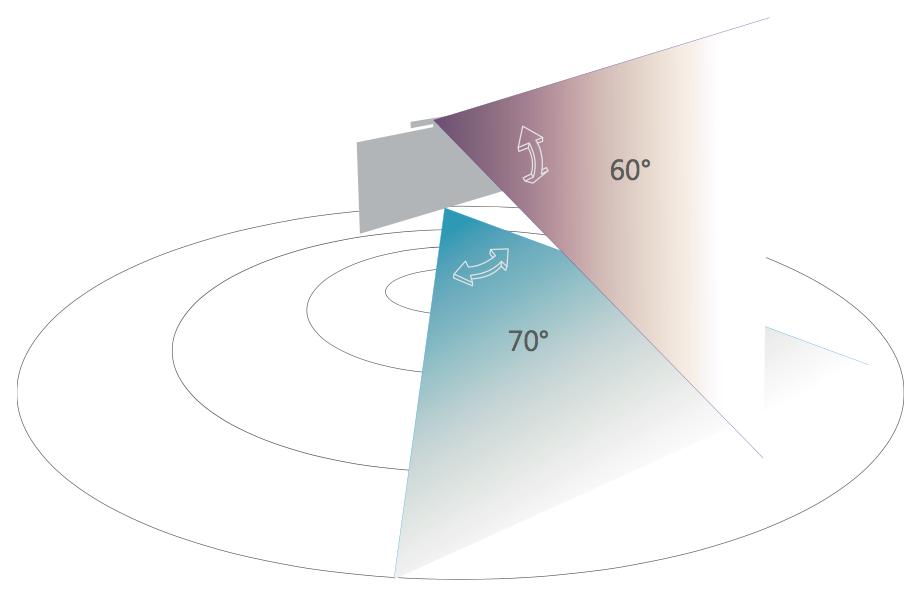
\includegraphics[width=1\linewidth]{Pictures/5_1_1_visionAngle}
		\subcaption{Angle of vision}
		\label{fig:5_1_1_visionAngle}
	\end{minipage}
	\hfill
	\begin{minipage}[t]{0.44\linewidth}
		\centering
		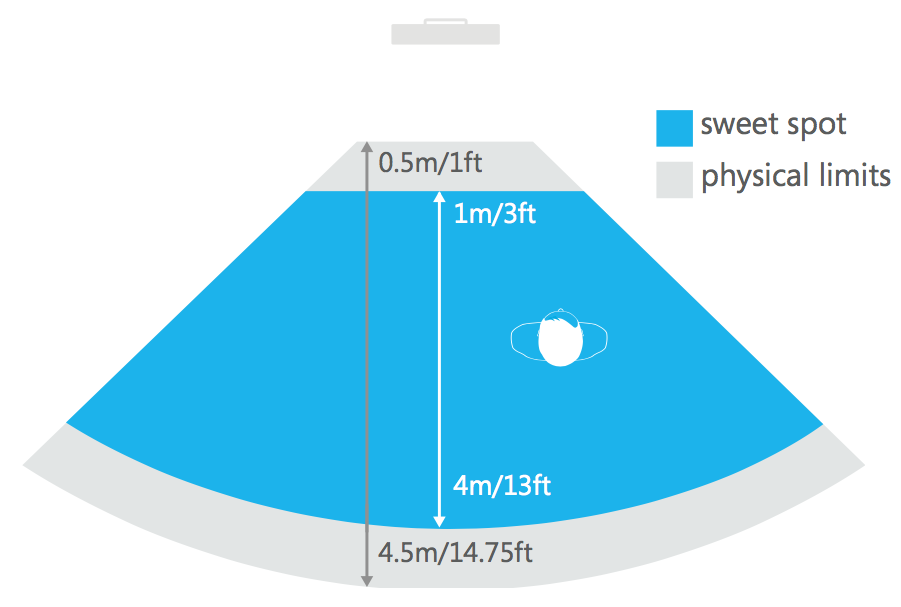
\includegraphics[width=1\linewidth]{Pictures/5_1_1_trackingRange}
		\subcaption{Kinect tracking range}
		\label{fig:5_1_1_trackingRange}
	\end{minipage}
	\caption{Sensor constraints of the Kinect v2~\cite{MicrosoftHIG2014-mh}}
	\label{fig:5_1_1_sensorConstraints}
\end{figure}

\subsection{Testing scenario}

%The test took place in the laboratory of the research group in the \textit{german reasearch center for artificial intelligence}~\footnote{\url{https://www.dfki.de/web/kontakt/dfki-saarbruecken}}. A big advantage of this is the large space to place the slackline easily in different variations. 
The slackline is placed in three positions to the Kinect: frontal (0 Degree), diagonal (45 Degree) and sideways (90 Degree) \textbf{\todo{(Figure X - 1)}}. Each of this positions is tested regarding three different height level of the Kinect: 80 cm, 160 cm, and 240 cm. Therefore it was attached on a tripod or traverse system (\textbf{\todo{Figure X - 2}}). At the end nine different combinations are covered to track a user on a slackline, which gives a general overview of the Kinect height to the slackline. The testing person was recorded via \textit{KinectStudio}~\footnote{\url{https://developer.microsoft.com/de-de/windows/kinect/tools}}, a tool for recording clips out of the streaming data of the Kinect. In the following the results discuss the feasibility and appropriate tracking positions.

\subsection{Slackline \& Kinect positioning}
With a slackline positioned sideways in 90 Degrees rotated to the Kinect, the advantage is that the whole body on the slackline is in a constant line within the tracking area. No interference regarding the limits of the tracking range can happen \textbf{\todo{(Figure X)}}. However, the Kinect had problems to detect the body joints with appropriate accuracy and precision, because of overlapping body parts (\textbf{\todo{Figure X}}).

By placing the slackline diagonal in 45 Degrees to the Kinect the frontal and end point of the slackline now differ in the vertical axis, which is unproblematic  \textbf{\todo{(Table X and Figure X)}}. 
%This could even result in a better trackability in matter of the depth field range, since the distance in the front shrinked and is therefore closer to the Kinect depth view. 
It shows better results in tracking ability than the former positioning, because many body parts will not overlap. But it occurs that joints of the arms interfere with other body joints, especially at the end of the line. Also both legs occlude while stepping forwards \textbf{\todo{(Figure X)}}. 
%This results in a relatively bad skeletal tracking and depending on the executed exercise it can lead to detection problems.

Positioning the slackline frontal towards the Kinect resulted in the best user tracking.
The sensor can see the full body and track the joints without any problems.
But detection failure occurred at the starting position of the slackline since the it utilises the entire depth range of the Kinect. This is because the user stands closer to the outermost limit of the detection range~\textbf{\todo{(Figure X)}}.

%Three main height levels were used to show the main differences of the tracking behaviour from the Kinect. It is mounted on a tripod and covers the heights of 0.80, 1.60 and 2.40 meters off the ground. 

Beginning with a height of 2.40 meters the Kinect has a very steep view angle to track the slackers' body on the full range of the slackline. Because of this the depth range shifts into the front like seen in \textbf{\todo{Figure X}}. Therefore, if the slacker begins at the starting position on the slackline, she immediately reaches the end of the tracking area which can cause detection problems. Also the closer she walks towards the Kinect the more the joints overlap due to the angle view of the Kinect.

With a height of 1.60 and 0.80 meters the entire body is fully visible in almost all ranges. The Kinect has a relatively flat angle. This results in a more homogeneous depth range ( \textbf{\todo{Figure X}}). Problems can occur at the very end of the slackline depending on the persons' height, which leads to cropped body parts like the head or arms. The slackline must be positioned slightly further away from the Kinect camera to prevent this.

\todo{\textbf{table}}
%The tracking and view is more homogeneous and the angle flatter, which results in the possibility to use the full depth range. With a higher attachment the angle will be too steep, which results in less depth range, as well as more occlusions of body parts can occur.
\rowcolors{2}{tablerowgray}{tablerowgray}
\begin{table}[h!]
\centering
%\arrayrulecolor{white}
\renewcommand{\arraystretch}{1}
\begin{tabular}{ | c | c | c | c | c | c | c | c | }
\hline
\rowcolor{tableheadergray} & \multicolumn{7}{ c| }{\textbf{Slackline Positioning}} \\ 
\rowcolor{tableheadergray} & \multicolumn{2}{ c| }{\textbf{Frontal}} & \multicolumn{2}{ |c| }{\textbf{Diagonal}} & \multicolumn{3}{ |c| }{\textbf{Sideways}}\\
\rowcolor{tableheadergray} \multirow{-3}{*}{\textbf{Kinect Height}} & \textbf{Front} & \textbf{Back} & \textbf{Front} & \textbf{Back} & \textbf{Front} & \textbf{Back} & \textbf{Mid} \\
\hline
2,40 m & 1,30m & 4,30m & 1,90m & 3,80m & 3,00m & 3,00m & 2,70m \\
\hline
1,60 m & 1,70m & 4,70m & 2,10m & 4,00m & 3,00m & 3,00m & 2,70m \\
\hline
0,80 m & 1,30m & 4,30m & 1,90m & 3,80m & 2,60m & 2,60m & 2,10m \\
\hline
\end{tabular}
\caption{Demographic data and physical activity table}
\label{table:1}
\end{table}

\subsection{Best positioning for study purposes}
% But since beginner will use the entire slackline range it can be neglected.
The best combination resulted placing the slackline frontal and having a Kinect height of 0.80 up to 1.60 meters. The Kinect can track the entire body with nearly no joint overlap. Since the focus of the study in this thesis lies mainly on beginners, the starting position of the slackline plays an important role. Hence, it is better to move the slackline closer to the camera because the very end of the line is not important for the study.
%a little bit of slackline is cropped out of the view but 
With this a higher tracking confidence is possible at the starting position, which is more important in this case \textbf{\todo{(Figure X)}}.
%This results in a relatively bad skeletal tracking and depending on the executed exercise it can lead to detection problems.